\documentclass[12pt]{article}
\usepackage{amssymb}
\usepackage{amsmath}
\usepackage{mathtools}
\usepackage[utf8]{inputenc}
\usepackage{hyperref}
\usepackage{comment}
\usepackage{polski}
\usepackage{mathrsfs}
\usepackage{geometry}
\usepackage{amsthm}
\usepackage{csquotes}
\usepackage{float}
\geometry{a4paper, portrait, margin=1in}

\usepackage[breaklinks=true]{hyperref}
\usepackage{subcaption}

\setlength\parindent{0pt}

\DeclarePairedDelimiter\abs{\lvert}{\rvert}%
\DeclarePairedDelimiter\norm{\lVert}{\rVert}%

% Swap the definition of \abs* and \norm*, so that \abs
% and \norm resizes the size of the brackets, and the 
% starred version does not.
\makeatletter
\let\oldabs\abs
\def\abs{\@ifstar{\oldabs}{\oldabs*}}
%
\let\oldnorm\norm
\def\norm{\@ifstar{\oldnorm}{\oldnorm*}}
\makeatother

\newcommand{\Cov}{\mathrm{Cov}}
\newcommand{\corr}{\mathrm{corr}}
\newcommand{\pH}{\mathscr{H}}
\newcommand{\bH}{\mathscr{B}(\mathscr{H})}
\newcommand{\gH}{\mathscr{G}(\mathscr{H})}
\newcommand{\complex}{\mathbb{C}}
\newcommand{\real}{\mathbb{R}}
\newcommand*\conj[1]{\overline{#1}}
\newcommand*\dotprod[2]{\langle #1 , #2 \rangle}
\newtheorem{theorem}{Twierdzenie}[section]
\newtheorem{corollary}{Wniosek}[theorem]
\newtheorem{lemma}[theorem]{Lemat}
\newtheorem{fact}[theorem]{Fakt}
\newtheorem{definition}[theorem]{Def.}
\newtheorem{example}[theorem]{Pd.}
\newcommand{\pder}[2][]{\frac{\partial#1}{\partial#2}}
% Command for partial derivatives. The first argument denotes the function and the second argument denotes the variable with respect to which the derivative is taken. The optional argument denotes the order of differentiation. The style (text style/display style) is determined automatically
\providecommand{\pd}[3][]{\ensuremath{
\ifinner
\tfrac{\partial{^{#1}}#2}{\partial{#3^{#1}}}
\else
\dfrac{\partial{^{#1}}#2}{\partial{#3^{#1}}}
\fi
}}

\title{Projekt II - finite difference and uncertain parameters.}
\author{Wojciech Fica \footnote{\href{mailto:wojtekfica@gmail.com}{wojtekfica@gmail.com}}, Krzysztof Krawiec \footnote{\href{mailto:TODO}{TODO}}, Wojciech Prokopowicz \footnote{\href{mailto:TODO}{TODO}}}
\date{\today}

\begin{document}

\section{Sprawdzenie wyników}
Metoda finite-difference jest uznaną i sprawdzoną metodą wyceny opcji, ale zawsze istnieje szansa, że podczas implementacji popełniliśmy błąd. Aby nabrać przekonania co do prawdziwości otrzymanych wyników możemy użyć innych znanych nam metod wyceny, które może nie będą działały w takiej ogólności jak finite-difference, ale za to są nieco łatwiejsze w implementacji.

Wybrane metody wyceny opcji:
\begin{enumerate}
    \item Jawne wzory (spełniające równanie Blacka-Scholesa): istnieją dla europejskich opcji barierowych,
    \item Drzewo trójmianowe: metoda pozwala wycenić barierowe opcje europejskie i amerykańskie (możliwość wprowadzenia dywidenty procentowej),
    \item Metoda Monte Carlo: w swej podstawowej formie nadaje się do wyceny europejskich opcji barierowych z dywidentą procentową bądź kwotową.
\end{enumerate}

Należy zauważyć, że powyższe metody nie dają nam od razu całej siatki wyceny opcji, a jedynie jej wartość w chwili zero dla konkretnej wartości początkowej aktywa bazowego. Innym zaletą finite-difference jest możliwość wprowadzenia do modelu niepewnej zmienności, na co nie pozwalają pozostałe metody.

\subsection{Drzewo trójmianowe}

Model wyceny opcji barierowych za pomocą drzewa trójmianowego jest naturalnym rozszerzeniem metody drzewa dwumianowego. W tym wypadku zakładamy, że w każdym kroku czasu \(dt\) cena aktywa bazowego wykonuje albo skok do góry, albo w dół, albo pozostaje na tym samym poziomie. Wysokość skoków dobieramy zgodnie ze zmiennością i wielkością \(dt\) oraz tak aby bariera wypadła na jednym z poziomów cen aktywa (patrz Rysunek \ref{fig:tbt}). W ten sposób zapewniamy, że bariera stosowana podczas wyceny jest dokładnie taka jak ta zadana. 

\begin{figure}[H]
    \centering
    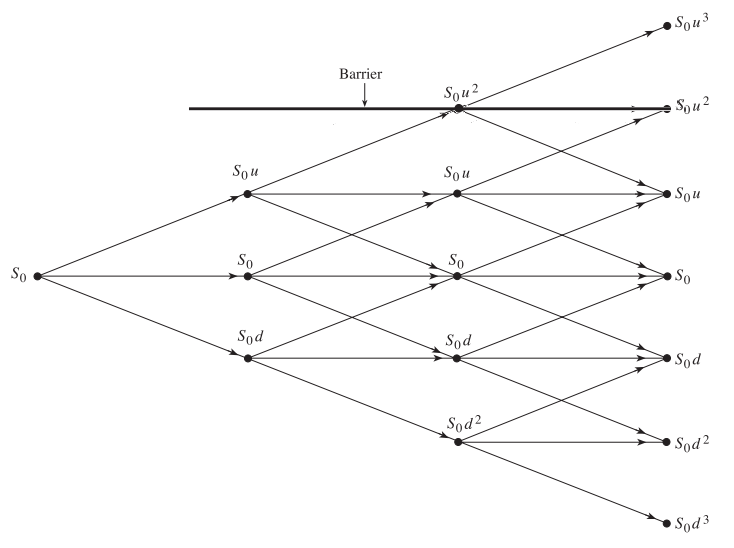
\includegraphics[width=0.75\textwidth,height=\textheight,keepaspectratio]{tbt.png}
    \caption{Drzewo trójmianowe}
    \label{fig:tbt}
\end{figure}

Prawdopodobieństwa przejść są tak dobrane aby ruchy cen akcji odpowiadały światowi neutralnemu na ryzyko. Wyceny dokonujemy dla kolejnych kolumn drzewa (podążając z prawej do lewej) w każdym wierzchołku wpisując wartość opcji odpowiadającą temu wierzchołkowi wyliczoną jako zdyskontowana wartość oczekiwana opcji w następnym kroku. 

Warto zauważyć, że łatwo możemy wprowadzić w tym modelu dywidendę procentową (ceny aktywa zaliczą spadek w momencie dywidendy), ale nie kwotową, ponieważ taki spadek spowoduje, że wierzchołki drzewa przestaną się rekombinować (sklejać) po momencie dywidendy.

\subsection{Opcje europejskie i amerykańskie bez dywidendy}

Dla ustalenia uwagi w tym rozdziale, jeśli nie zostanie stwierdzone inaczej będziemy rozważać następujące parametry opcji: 
\begin{itemize}
    \item cena wykonania: \(2100\),
    \item bariera dla opcji call: \(2400\),
    \item bariera dla opcji put: \(1900\),
    \item zmienność roczna: \(20\%\),
    \item stopa procentowa: \(1.5\%\).
\end{itemize}

Dokonujemy wyceny opcji na chwilę zero dla różnych wartości początkowych aktywa bazowego (\(S_{0}\)).

\begin{figure}[H]
    \centering
    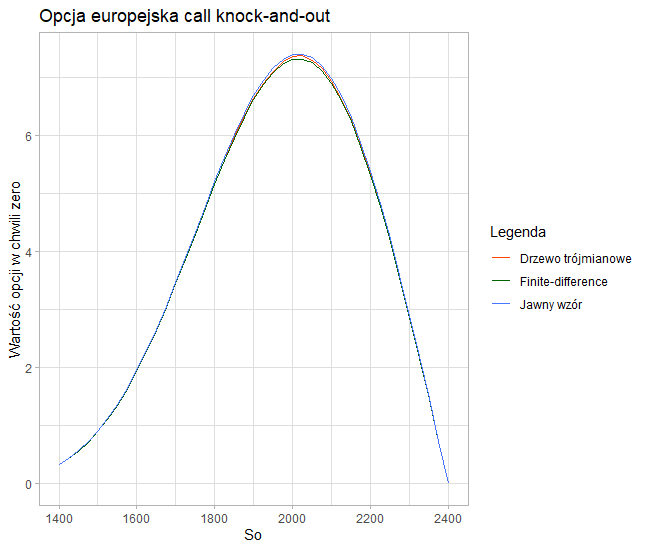
\includegraphics[width=0.8\textwidth,height=\textheight,keepaspectratio]{ec_porownanie.png}
    %\caption{Drzewo trójmianowe}
    \label{fig:ec}
\end{figure}

\begin{figure}[H]
    \centering
    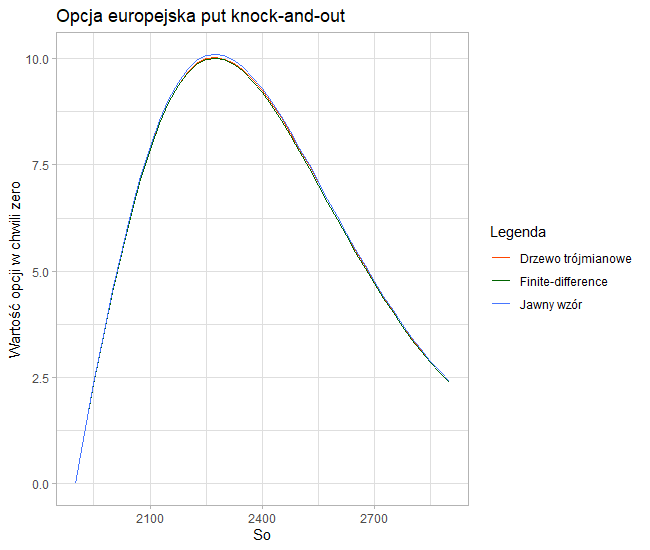
\includegraphics[width=0.8\textwidth,height=\textheight,keepaspectratio]{ep_porownanie.png}
    %\caption{Drzewo trójmianowe}
    \label{fig:ep}
\end{figure}

\begin{figure}[H]
    \centering
    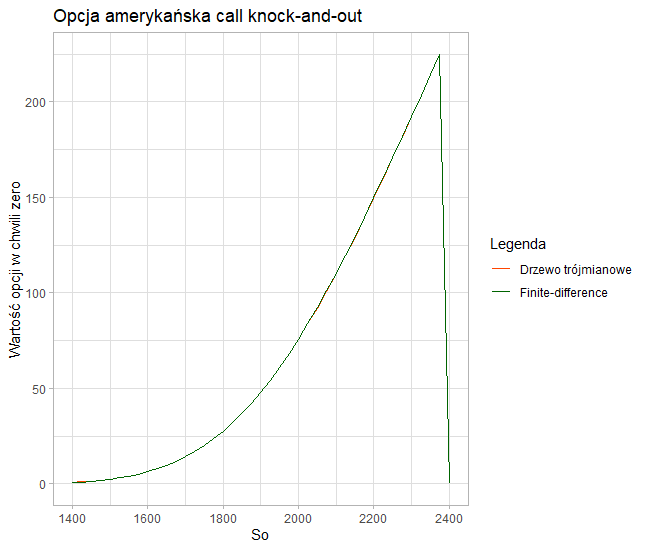
\includegraphics[width=0.8\textwidth,height=\textheight,keepaspectratio]{ac_porownanie.png}
    %\caption{Drzewo trójmianowe}
    \label{fig:ac}
\end{figure}

\begin{figure}[H]
    \centering
    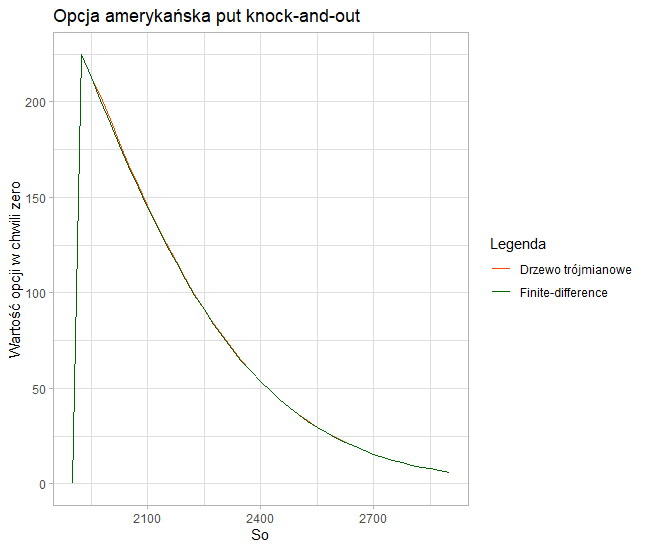
\includegraphics[width=0.8\textwidth,height=\textheight,keepaspectratio]{ap_porownanie.png}
    %\caption{Drzewo trójmianowe}
    \label{fig:ap}
\end{figure}

\begin{tabular}{c||c|c|c|c}
    Rodzaj opcji & EC & EP & AC & AP \\
    \hline
    Maksymalna różnica & 0.086 & 0.095 & 0.37 & 2.65
\end{tabular}\\

Widzimy, że nasze wyceny pokrywają się niemal idealnie. Oczywiście pokazaliśmy zgodność tylko dla jakichś przykładowych parametrów, ale szansa, że to nam się udało przez przypadek jest raczej znikoma. \\

Ważnym parametrem podczas wyceny była zmienność. Możemy zatem popatrzeć na wyceny opcji dla różnych wartości zmienności. Niech \(S_{0}\) dla opcji call wynosi \(2000\), a dla opcji put - \(2400\).

\begin{figure}[H]
    \centering
    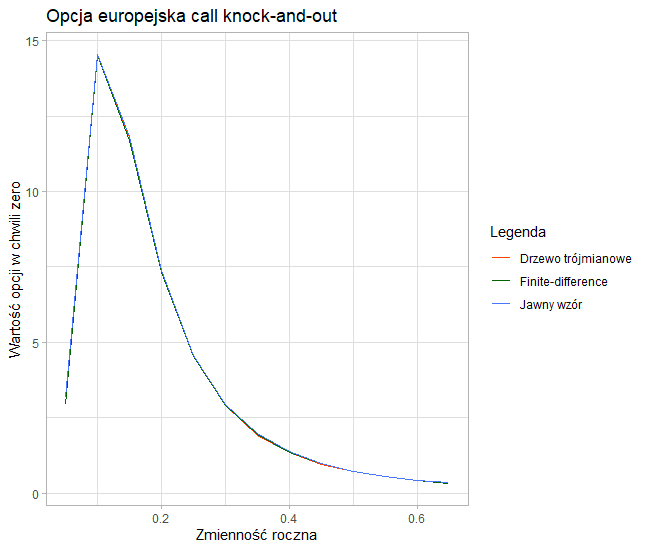
\includegraphics[width=0.8\textwidth,height=\textheight,keepaspectratio]{ec_sig_porownanie.png}
    %\caption{Drzewo trójmianowe}
    \label{fig:ecs}
\end{figure}

\begin{figure}[H]
    \centering
    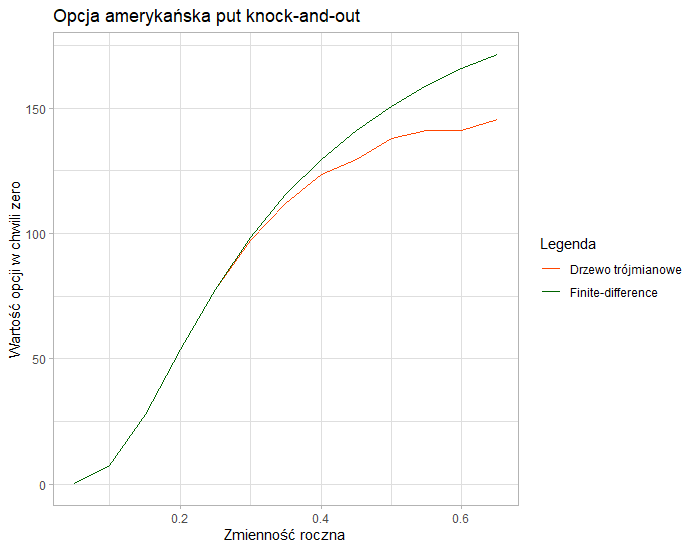
\includegraphics[width=0.8\textwidth,height=\textheight,keepaspectratio]{ap_sigma.png}
    %\caption{Drzewo trójmianowe}
    \label{fig:aps}
\end{figure}

Ponownie obserwujemy zgodność wycen. Jedyna rozbieżność zaczyna pojawiać się dla opcji amerykańskiej z wysoką zmiennością. Jest to spowodowane za małą liczbą kroków przy wycenie drzewem trójmianowym. Większa zmienność przekłada się na większe skoki cen aktywa, przez co następuje niedoszacowanie wartości opcji amerykańskiej (możliwość wczesnego wykonania tuż przed barierą). Zwiększenie liczby kroków w algorytmie powoduje zbliżenie się wyceny do finite-difference (w zamian algorytm staje się powolny).

\subsection{Metoda Monte Carlo}

Wartość opcji może być wyznaczona jako zdyskontowana wartość oczekiwana payoffu, jeśli trajektorie kursu aktywa będą modelowane przez geometryczny ruch Browna w świecie neutralnym na ryzyko, tzn. będą spełniały: \[dS=rSdt+\sigma SdX,\] gdzie \(X\) jest standardowym ruchem Browna. Wartość opcji wynosi wtedy: \[f=e^{-rT}E[payoff(S)].\]

Metoda Monte Carlo polega więc na tym, aby wygenerować \(M\) takich trajektorii obliczyć ich payoffy, wyciągnąć średnią i ją zdyskontować. Mocne Prawo Wielkich Liczb mówi nam, że tak otrzymana wartość \(\mu\) opcji będzie zbiegać do \(f\), gdy \(M\rightarrow \infty\). 

Ponadto możemy wyznaczyć przedział ufności, w którym \(f\) znajdzie się z prawdopodobieństwem \(95\%\): \[\Big( \mu - \frac{1.96\omega}{\sqrt{M}},\, \mu + \frac{1.96\omega}{\sqrt{M}}\Big),\] gdzie \(\omega\) jest odchyleniem standardowym z otrzymanych payoffów.

Metoda ta jest bardzo prosta w użyciu i łatwa w modyfikacji (np. wprowadzenie dywidendy), ciężej jest ją dostosować do wyceny opcji amerykańskich (nie będziemy tego robić). Największym mankamentem jest konieczność wygenerowania bardzo wielu trajektorii, aby uzyskać sensowny przedział ufności.

\subsection{Opcje z dywidendą}
W tym rozdziale zakładamy, że dywidenda jest wypłacana w połowie życia opcji.\\

W metodzie Monte Carlo generowaliśmy \(M=50000\) trajektorii, co dawało przedziały ufności (na poziomie istotności \(\alpha=0.05\)) nie dłuższe niż \(0.6\).

\begin{figure}[H]
    \centering
    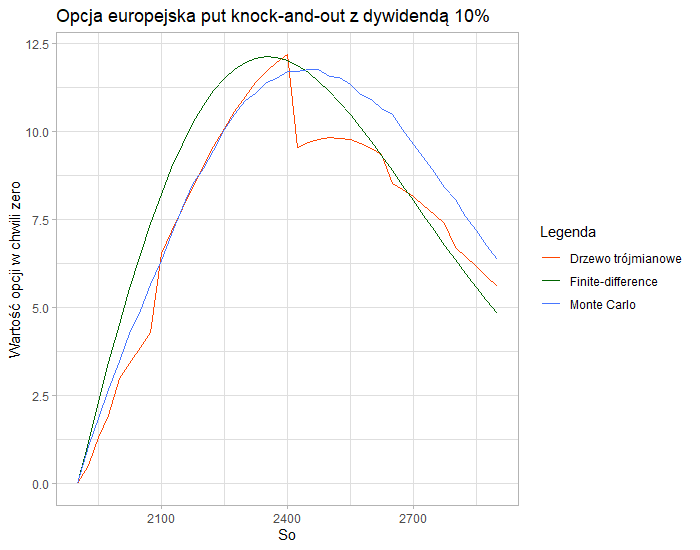
\includegraphics[width=0.8\textwidth,height=\textheight,keepaspectratio]{dyw10proc.png}
    \caption{}
    \label{d10}
\end{figure}

Na Rysunku \ref{d10} mamy przedstawioną wycenę opcji europejskiej put z dywidendą procentową trzema metodami. Choć nie pokrywają się już tak idealnie jak poprzednio, to nadal są to bardzo zbliżone wyceny. Widać jednak, że dywidenda wprowadziła dosyć gwałtowną zmianę w procesie wyceny, z którą różne metody różnie sobie poradziły. Zauważmy na przykład, że bariera w drzewie trójmianowym po momencie dywidendy nie musi już leżeć nie jakimś poziomie cen aktywa, na czym nam zależało.

\begin{figure}[H]
    \centering
    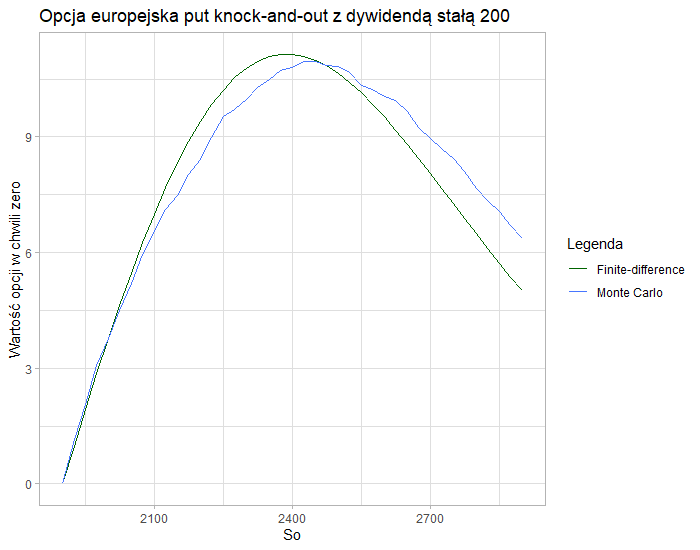
\includegraphics[width=0.8\textwidth,height=\textheight,keepaspectratio]{dyw200.png}
    \caption{}
    \label{d200}
\end{figure}

\begin{figure}[H]
    \centering
    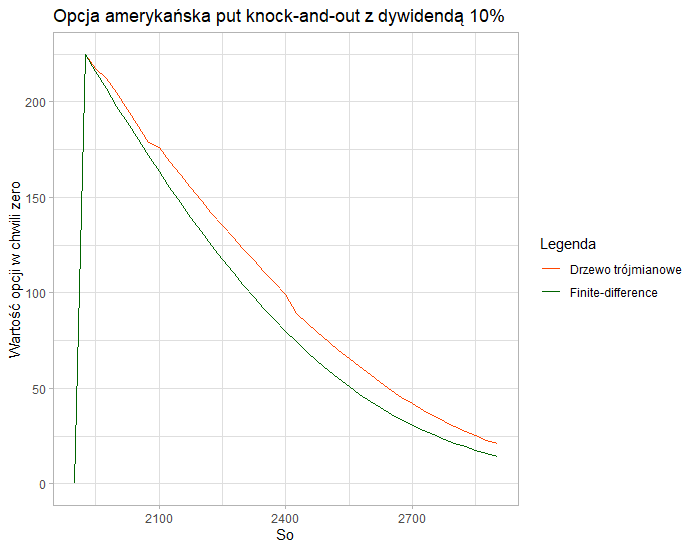
\includegraphics[width=0.8\textwidth,height=\textheight,keepaspectratio]{ap_dyw10.png}
    \caption{}
    \label{adyw}
\end{figure}

Rysunek \ref{d200} przedstawia porównanie dla dywidendy kwotowej, a Rysunek \ref{adyw} dla opcji amerykańskiej. Są to ponownie bardzo zbliżone wyniki. Niestety nie posiadamy zaimplementowanej metody, kora pomogłaby nam sprawdzić wycenę finite-difference opcji amerykańskiej z dywidendą kwotową.

\subsection{Warunki brzegowe}
Jeszcze innym sposobem aby upewnić się, że nie popełniło się błędu w trakcie implementacji jest sprawdzenie pewnych skrajnych przypadków, co do których mamy silne intuicje lub nawet pewność, jeśli chodzi o to, co powinno wyjść. 

\begin{figure}[H]
    \centering
    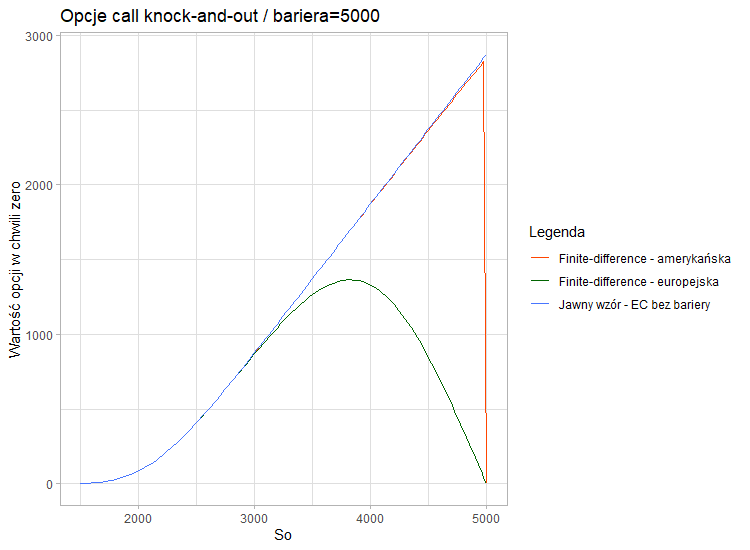
\includegraphics[width=0.8\textwidth,height=\textheight,keepaspectratio]{bariera5000.png}
    \caption{}
    \label{b5000}
\end{figure}

Rysunek \ref{b5000} pokazuje, co się dzieje jeśli odsuniemy barierę daleko od ceny wykonania. Zauważmy, że wycena europejskiej opcji barierowej dla wartości początkowych aktywa poniżej \(3000\) jest niemal identyczna jak wycena zwykłej opcji europejskiej.\\

\begin{figure}[H]
    \centering
    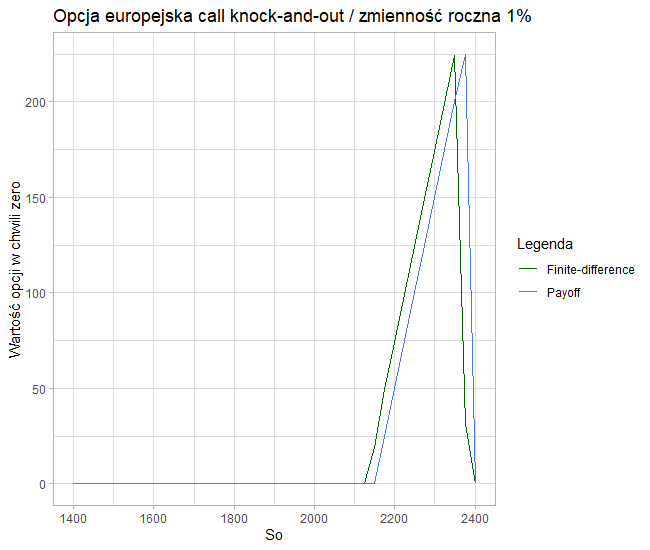
\includegraphics[width=0.8\textwidth,height=\textheight,keepaspectratio]{ec_sigma0.png}
    \caption{}
    \label{sigma0}
\end{figure}

Rysunek \ref{sigma0} ma za to obrazować, co się dzieje, gdy zmienność roczna zbliża się do zera. Można o tym myśleć w ten sposób, że sytuacja, w której mamy małą zmienność roczną jest analogiczna do sytuacji, w której zmienność jest większa, ale za to znajdujemy się blisko momentu wykonania, tzn. jest mało czasu na to aby cena aktywa znacznie się zmieniła. Z tego powodu wycena opcji jest bardzo zbliżona do payoffu.\\

Nasze intuicje oraz wyceny innymi metodami zgadzają się z otrzymanymi wynikami dla finite-difference, zatem możemy przypuszczać, że nasza implementacja jest poprawna.

\end{document}